\documentclass[12pt]{report}
\usepackage[T2A]{fontenc} 
%\usepackage[cp1251]{inputenc}
\usepackage[utf8]{inputenc}
\usepackage[russian, english]{babel}
\usepackage{cmap}
\usepackage{xkeyval}
\usepackage[pdftex]{graphicx}
\usepackage{amsmath}
\usepackage{amsfonts}
\usepackage{multirow}
\usepackage{xfrac}
\usepackage[labelformat=empty]{caption}
\usepackage[left=2cm,right=2cm,
     top=2cm,bottom=2cm,bindingoffset=0cm]{geometry}
     %\geometry{margin=1cm}%Just for showing, these are bad margins!
%\usepackage[pdftex]{graphics}
\graphicspath{{images/}}
\frenchspacing

%4 listing 

\usepackage{listings} %% собственно, это и есть пакет listings
\usepackage{color} %% это для отображения цвета в коде
\definecolor{mygreen}{rgb}{0,0.6,0}
\definecolor{mygray}{rgb}{0.5,0.5,0.5}
\definecolor{mymauve}{rgb}{0.58,0,0.82}
\tolerance=1000

\usepackage{caption}
\DeclareCaptionFont{white}{\color{white}} %% это сделает текст заголовка белым
%% код ниже нарисует серую рамочку вокруг заголовка кода.
\DeclareCaptionFormat{listing}{\colorbox{black}{\parbox{\textwidth}{#1#2#3}}}
\captionsetup[lstlisting]{format=listing,labelfont=white,textfont=white}

\usepackage{etoolbox}
\makeatletter
\patchcmd{\chapter}{\if@openright\cleardoublepage\else\clearpage\fi}{}{}{}
\makeatother


\begin{document}

\righthyphenmin=2
\newpage
\hfill \text{Серебро Андрей, студент  43601/2}\\

\section* {Решённые задачи}
\parindent=1cm
\newenvironment{myindentpar}[1]%
 {\begin{list}{}%
         {\setlength{\leftmargin}{#1}}%
         \item[]%
 }
 {\end{list}}
 
\subsection*{Нумерация двумерных диаграмм}
\hspace{\parindent} Повторены результаты предшественников по части нумерации двумерных диаграмм Юнга. 

Обозначим: 

\begin{itemize}
  \item $\No(\lambda)$  - номер диаграммы $\lambda$
  \item $Cells(\lambda)$  - число клеток в $\lambda$
  \item $h_Y(i)$ - высоту столбца с номером $i$ в диаграмме $\lambda$ (высоты считаем положительными целыми числами)
  \item $r_Y(i)$ - длину строки с номером $i$ в диаграмме $\lambda$
  \item $Cols(\lambda)$ - число столбцов в диаграмме $\lambda$
\end{itemize}
Нумерация удовлетворяет следующим трём правилам:\\
1. Номер диаграммы из одной клетки равен 1;\\
2. Если $Cells(\lambda_1) < Cells(\lambda_2)$, то $\No(\lambda_1) < \No(\lambda_2)$;\\
3. Иначе если $Cells(\lambda_1) = Cells(\lambda_2)$ и $\exists k \ge 1 : \forall i \in \{1..k-1\} h_{\lambda_1}(i) = h_{\lambda_2}(i)$ и $h_{\lambda_1}(k) < h_{\lambda_2}(k)$, то $\No(\lambda_1) < \No(\lambda_2)$

Для того, чтобы найти номер диаграммы по этим правилам, предварительно подсчитывается $P(n, k)$ $\forall n, k \in \mathbb{N} : 0 < n < N, k < n$ - число разбиений числа $n$ на натуральные слагаемые с максимальным слагаемым, не превосходящим $k$. На данный момент число $N = 600$, так как нумерация диаграмм с большим числом клеток не требуется. Далее, для нахождения номера диаграммы, применяется Алгоритм 1.
\vspace{1cm}

Алгоритм 1 (получения номера диаграммы).

ВХОД: диаграмма $\lambda$, заданная высотами столбцов.

ВЫХОД: $\No(\lambda)$.

1. $num := 1, c := 1$ 

2. WHILE $c < Cells(\lambda)$ DO 

\hspace{1cm} $num := num + P(c, c)$

\hspace{1cm} $c := c + 1$

\hspace{0.35cm} END WHILE

3. FOR i FROM 1 TO $Cols(\lambda)$ DO

\hspace{1cm} IF $h_\lambda(i) = 1$

\hspace{2cm} BREAK

\hspace{1cm} $num := num + P(c, h_\lambda(i) - 1)$

\hspace{1cm} $c := c - h_\lambda(i)$

\hspace{0.35cm} END FOR

4. RETURN num

Оценим сложность данного метода. Пусть требуется найти номер диаграммы из $n$ клеток. $P(n, n)$ растёт как $O(\frac{exp(\sqrt(n))}{n})$, поэтому длина номера $num$ в ходе цикла WHILE растёт как $O(\sqrt{c})$, поэтому сложность этого цикла не превосходит $O(n\sqrt{n})$. Цикл FOR также требует $O(n\sqrt{n})$ времени, поэтому весь алгоритм в худшем случае исполняется за $O(n\sqrt{n}$.

\subsection*{Точный подсчёт вероятностей диаграмм}

\hspace{\parindent} Для нескольких марковских процессов на графе Юнга реализован точный подсчёт вероятностей получения диаграмм с заданным числом клеток. Сейчас присутствуют процесс Ричардсона, Планшереля, псевдопланшерелевский процесс (переходная вероятность пропорциональная $(x^2+y^2)^{0.16}$), а также псевдоричардсонский процесс (переходная вероятность пропорциональна числу исходящих дуг из вершины, переходную вероятность в которую мы считаем). 

Точные вероятности для процесса Ричардсона удается быстро посчитать для диаграмм из 70-80 клеток. Для псевдопланшерелевского процесса за короткое время для диаграмм из 70 клеток. Предельная форма псевдоричардсоновского процесса совпадают с ричардсоновским (проверено в серии экспериментов, в которых строились случайные диаграммы из 100 000 клеток).

\subsection*{Предельные формы диаграмм}

\hspace{\parindent} Для описанных выше процессов построены предельные формы (брались диаграммы из 1000 000 клеток). Странно, что псевдопланшерель получился не похож на Планшереля - видимо, в Планшереле закралась ошибка, в связи с чем далее следует мой вопрос.

ВОПРОС: правильно ли я понимаю, что процесс Планшереля характеризуется как процесс, при котором вероятность любого пути до данной диаграммы $\lambda$ есть $P_{path} = \frac{dim\lambda ^2}{n!}$, поэтому, чтобы найти переходные вероятности из данной диаграммы в диаграммы следующего уровня графа, следует считать, что они просто пропорциональны числу таблиц Юнга для диаграммы, в которую рассчитывается вероятность перехода из данной: $P_{\lambda \rightarrow \lambda_i} \sim dim\lambda_i^2$? 

\begin{figure}[!ht]
\begin{center}
\includegraphics[scale=0.6]{howIUnderstand}
\\Рис. 1. Картинка по поводу вопроса.
\end{center}
\end{figure}

\begin{figure}[!ht]
\begin{center}
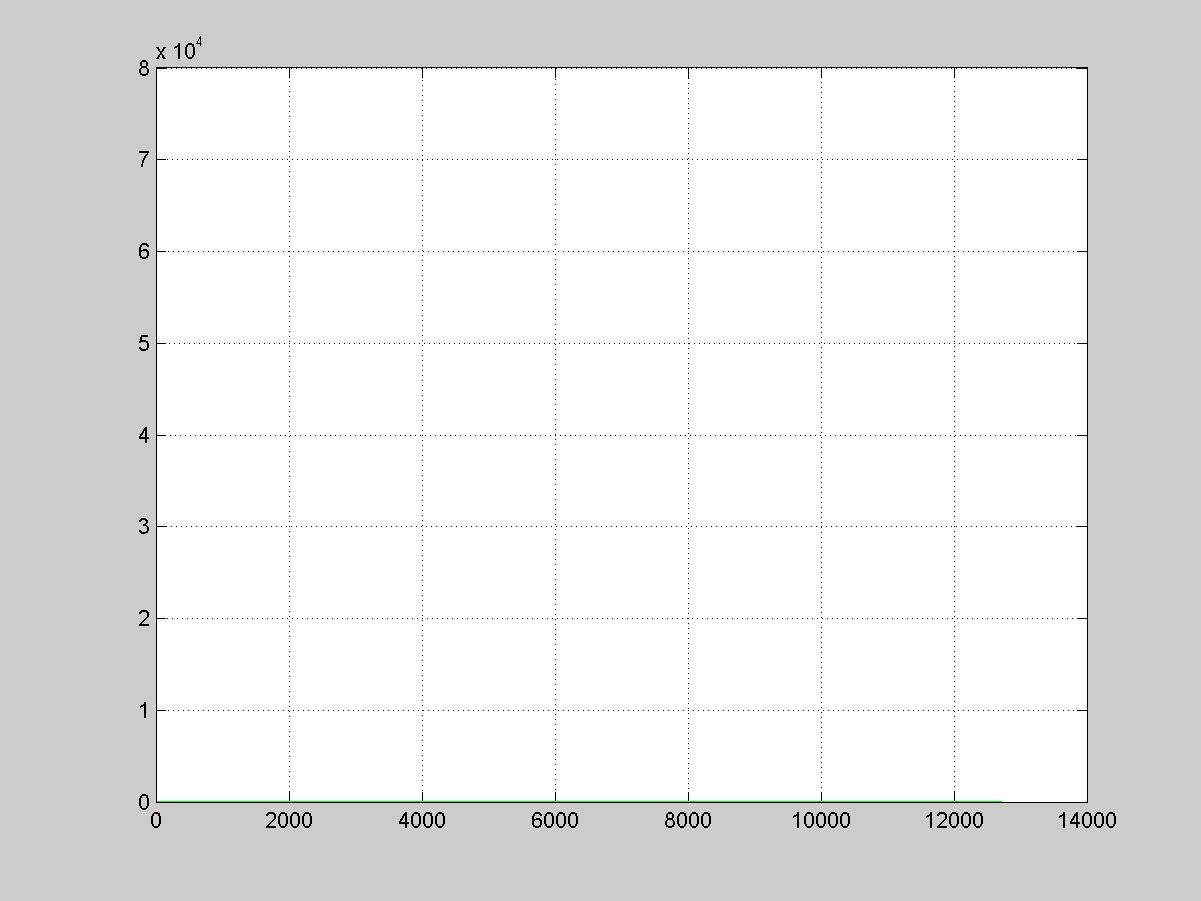
\includegraphics[scale=0.2]{Plansherel_assympt}
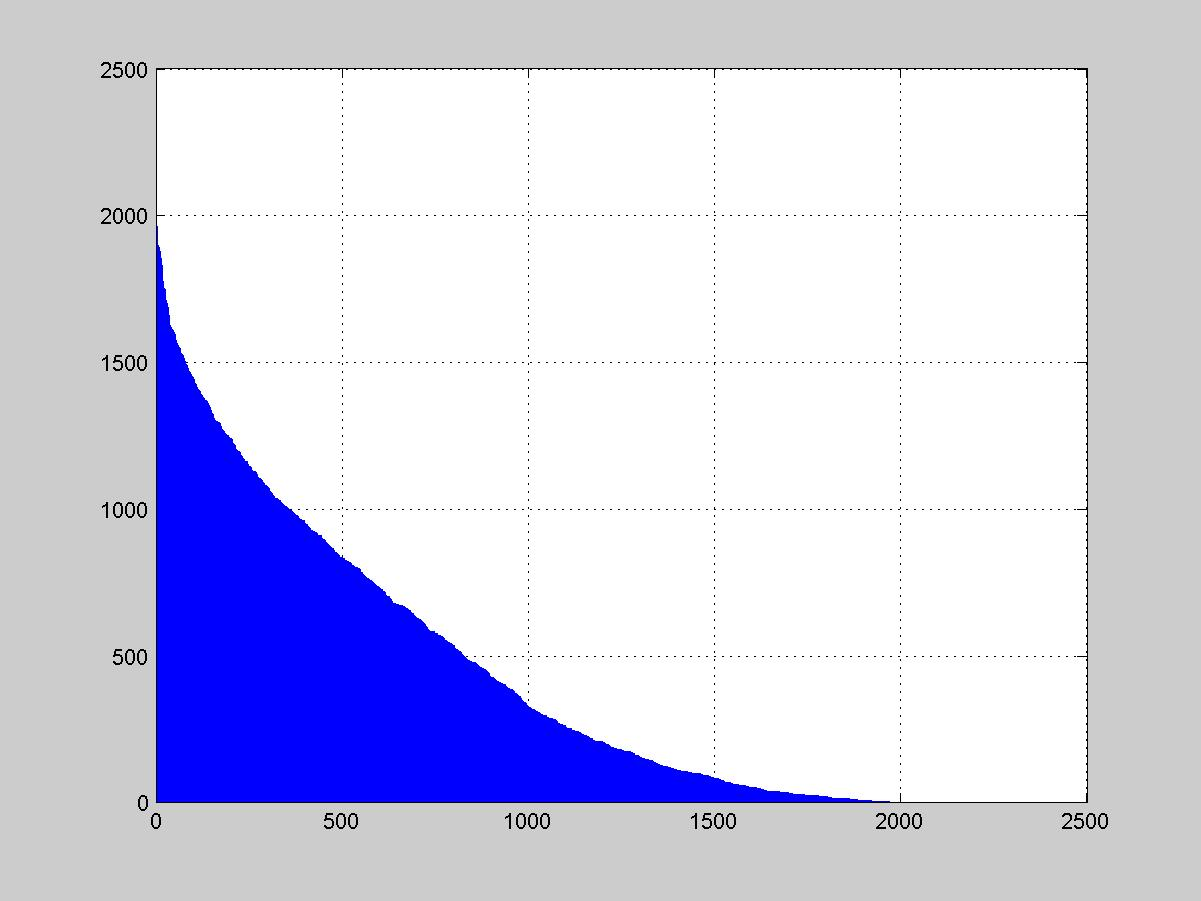
\includegraphics[scale=0.2]{ALPHA_assympt}
\\Рис. 2. Асимптотическая форма случайной диаграммы при процессе Планшереля (слева) и псевдоплашереля (справа).
\end{center}
\end{figure}

\begin{figure}[!ht]
\begin{center}
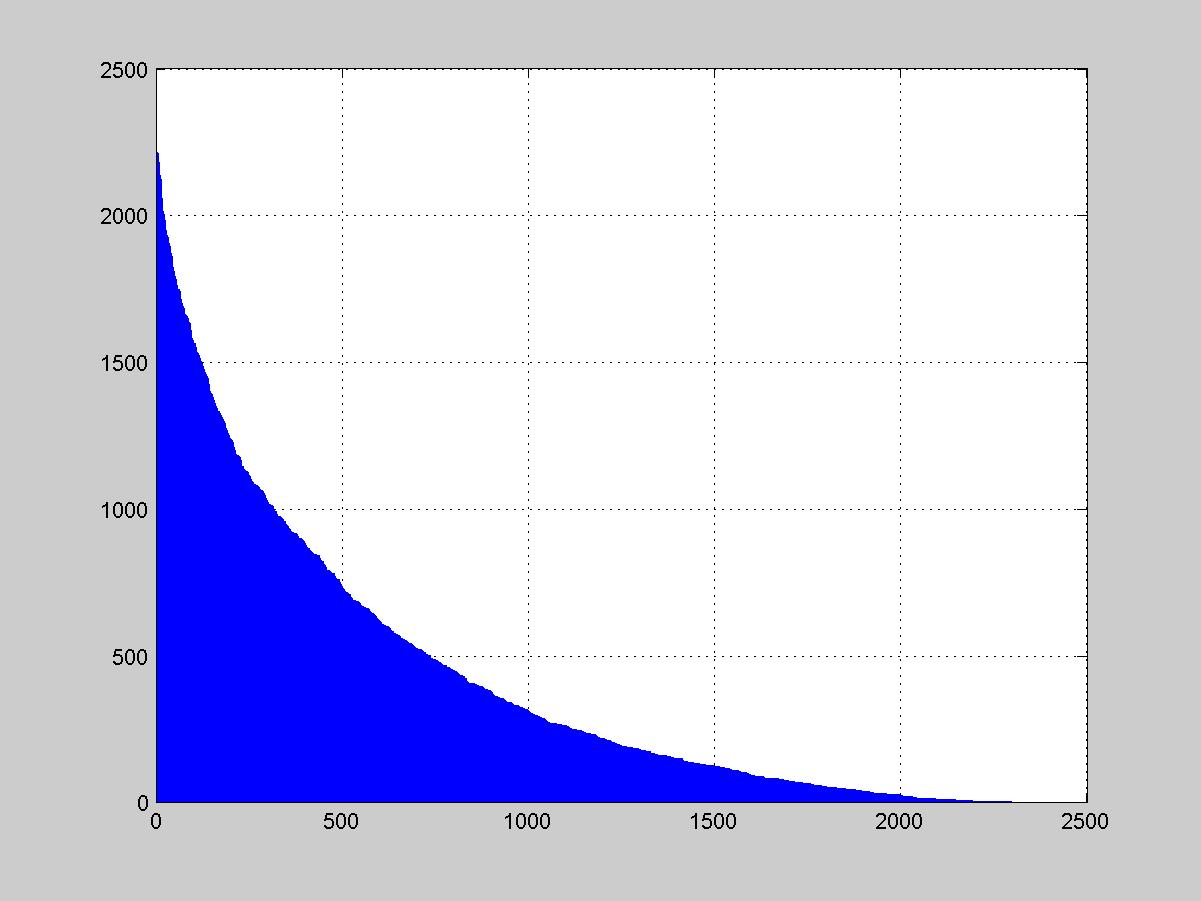
\includegraphics[scale=0.2]{Richardson_assympt}
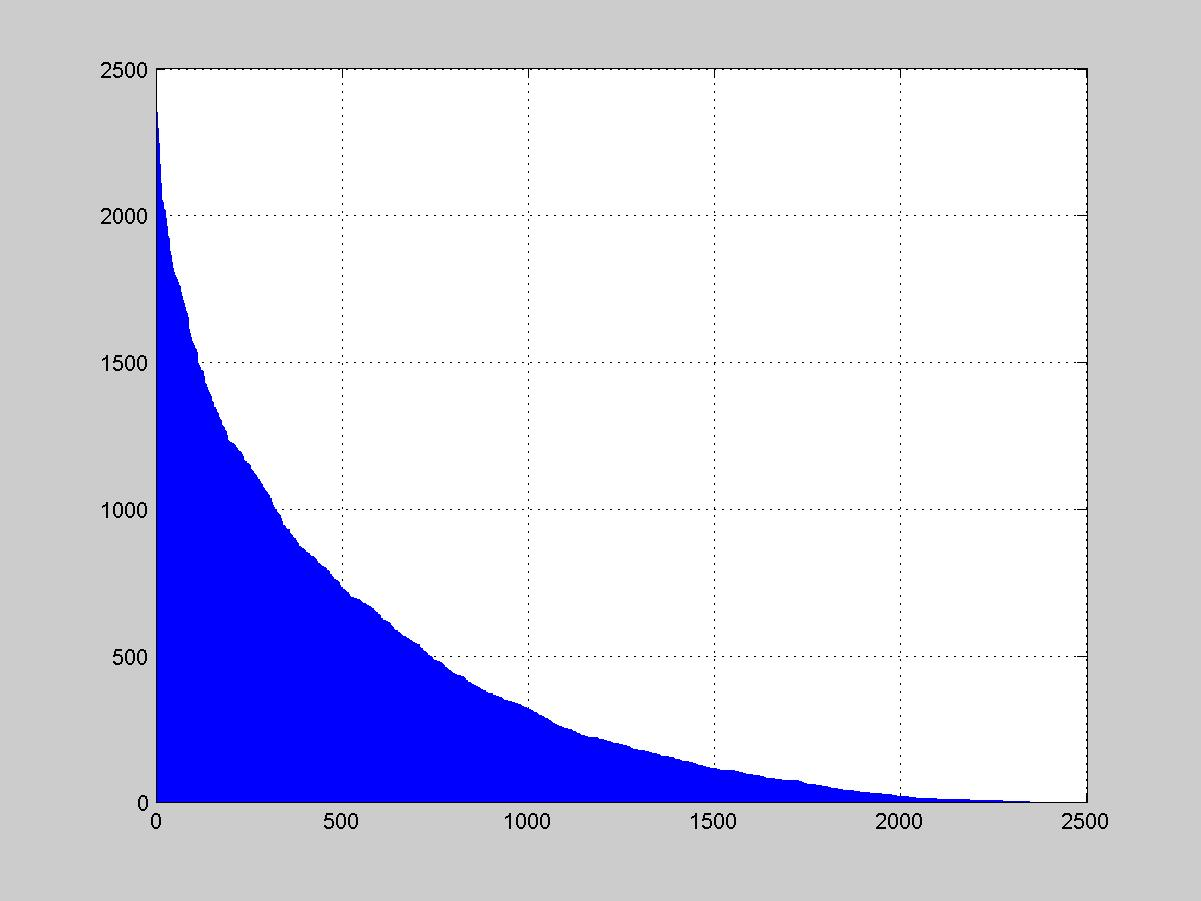
\includegraphics[scale=0.2]{Beta_assympt}
\\Рис. 3. Асимптотическая форма случайной диаграммы при процессе Ричардсона и псевдоричардсона.
\end{center}
\end{figure}

\newpage
\subsection*{Подсчёт расстояния Канторовича между диаграммами}

\hspace{\parindent} Основываясь на статье А. М. Вершика, реализован подсчёт расстояний Канторовича между диаграммами в графе Юнга. В качестве центральной меры на пространстве путей взята мера Планшереля. Проведены эксперименты (в том числе, я выяснил, что за разумное время - около получаса - можно найти расстояние между диаграммами из 50 клеток, при этом пришлось решить 36 695 768 транспортных задач.) Между диаграммами из 40 клеток расстояние ищется за время порядка 30 секунд. Также вычислены все расстояния между диаграммами на 10 этаже графа Юнга, гистограмму расстояний можно увидеть на рис. 4.

\vspace{1cm}

Алгоритм 2 (нахождения расстояния Канторовича между двумя вершинами с одного уровня градуированного графа).

ВХОД: две вершины $d_1, d_2$ одного уровня градуированного графа $G$.

ВЫХОД: $dist(d_1, d_2)$ - расстояние Канторовича между ними.

1. Создаём ассоциированный массив $distances[u, v]$, который будет содержать найденные расстояния между веришнами. Задаём расстояния на первом неединичном этаже графа и записываем их в этот массив (на первом этаже, содержащем больше одной вершины). Обозначим номер этого этажа через $s$.

2. Строим массивы вершин $V_i$ - предшественниц для $d_1$ и  $d_2$ с этажа $s \le i \le Cells(d_1)$ - для общности кода считаем вершины сами себе прдешественниками тоже. Попутно помечаем в каждой вершине поле $V.anc$, указывающее, какой вершине - $d_1$ или $d_2$ - она приходится предком. Если она приходится предком для обеих вершин, также отмечаем это (для этого с каждой вершиной достаточно ассоциировать два бита). 

3. FOR $i$ FROM $s + 1$ TO $Cols(d_1)$ DO

\hspace{1cm} FOR $v \in V_i$ DO

\hspace{2cm} $c_1 := \emptyset$

\hspace{2cm} $pred_1 := \emptyset$

\hspace{2cm} countCoefficientsForKantorovichMetric($v, c_1, pred_1$)

\hspace{2cm} FOR $u \in V_i$ DO

\hspace{3cm} IF $u.anc$ = $v.anc$ AND $u.anc$ XOR 3 = TRUE 

\hspace{4cm} CONTINUE

\hspace{3cm} $c_2 := \emptyset$

\hspace{3cm} $pred_2 := \emptyset$

\hspace{3cm} $costs := \emptyset$

\hspace{3cm} countCoefficientsForKantorovichMetric($u, c_2, pred_2$)

\hspace{3cm} FOR $p \in pred_1$ DO

\hspace{4cm} FOR $q \in pred_2$ DO

\hspace{5cm} $costs[p, q] := distances[p, q]$ 

\hspace{3cm} $x := $ solveTransportationPotential($costs, c_1, c_2$)

\hspace{3cm} $distances[u, v] := 0$

\hspace{3cm} FOR $p \in pred_1$ DO

\hspace{4cm} FOR $q \in pred_2$ DO

\hspace{5cm} $distances[u, v] := distances[u, v] + costs[p, q] \cdot x[p, q]$ 

\hspace{1cm} END FOR

\hspace{0.35cm} END FOR

4. RETURN $distances[d_1, d_2]$

\vspace{1cm}

Здесь используется функция countCoefficientsForKantorovichMetric($u, c, pred$), принимающая на вход вершину графа $u$ и возвращающая в массиве $c$ копереходные вероятности для рёбер, соединяющих $u$ c её предшественниками, а в $pred$ соответствующих предшественников $u$. Фунция solveTransportationPotential решает транспортную задачу методом потенциалов. Алгоритм оптимален в том смысле, что не вычисляет расстояния, которые не требуются для определения итогового расстояния.

Сложность данного алгоритма ещё предстоит оценить. Пока что очевидно, что число решаемых транспортных задач (скорее всего) в случае гарфа Юнга зависит от числа клеток во входных диаграммах экспоненциально. То есть, вряд ли граф Юнга достаточно локален, чтобы число предшественников не росло быстро. 

\begin{figure}[!ht]
\begin{center}
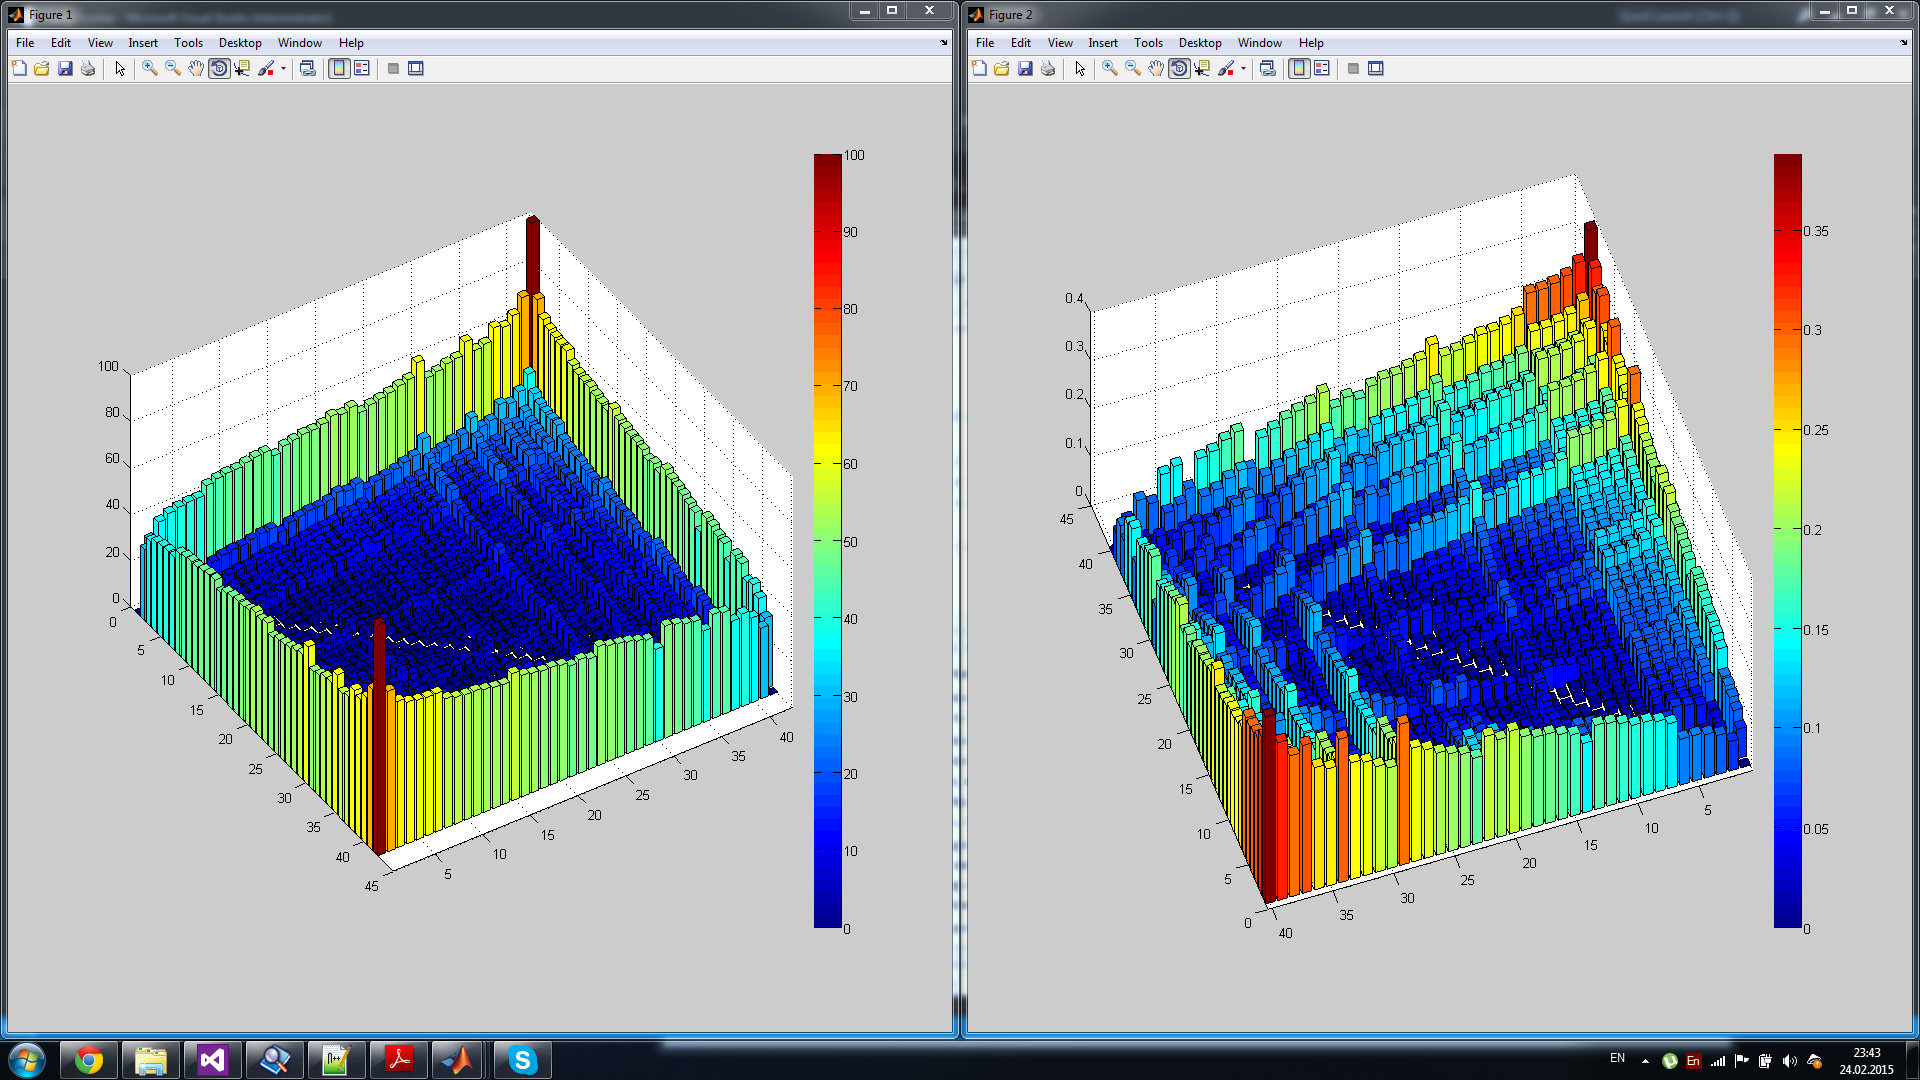
\includegraphics[scale=0.3]{metric}
\\Рис. 4. Гистограмма расстояний Канторовича между диаграммами 10го этажа графа Юнга. Правая картинка отражает расстояния между всеми диаграммами, кроме крайних, ибо они являются резкими выбросами и сглаживают картину для остальных.
\end{center}
\end{figure}

\section* {Нерешённые задачи}

\subsection*{Предельная форма трёхмерных диаграмм}
\hspace{\parindent} Николай Николаевич говорит, что было бы неплохо посмотреть, что будет, если использовать трёхмерный аналог формулы крюков для определения вероятностей перехода в трёхмерном случае (это уже будет не Планшерелевский процесс, ибо эта формула крюков в трёхмерном случае не даёт равновероятное появление любого пути до диаграммы). Попробовать возводить эти веса для переходных вероятностей в некоторые степени и посмотреть, будет ли меняться предельная форма. Посмотреть, что за кривые высекаются предельной диаграммой на координатных плоскостях.

\subsection*{Предельная форма двухмерных диаграмм}

\hspace{\parindent} Посмотреть, что будет, если возводить веса, найденные для Планшерелевских переходных вероятностей в малую отрицательную степень. При нулевой степени мы получаем процесс Ричардсона (очевидно, все веса 1), при положительных, больших 1, вроде как получаем того же Планшереля (Планшерель соответствует 1). При степенях от 0 до 1, я не помню, чему это соответствует, скорее всего тоже Планшерелю (надо проверить!).

\subsection*{Гипотеза Вершика}
\hspace{\parindent} Гипотеза состоит в том, что расстояние Канторовича между диаграммами можно представить в виде $dist(\lambda_1, \lambda_2) = \sum\limits_{i=1}^{h}c_i\Delta_i$, где $h = \max(h_{\lambda_1}(1), h_{\lambda_2}(1))$, $\Delta_i = |r_{\lambda_1}(i) - r_{\lambda_2}(i)|$, $c_i$ - какие-то коэффициенты, причём быстро убывающие с ростом $i$. Предлагается, насколько я понял, попробовать подобрать их, а также убедиться, что коэффициенты действительно быстро убывают:  например, это можно увидеть, рассмотрев расстояние между прямоугольной диаграммой и треугольной, которое видимо будет маленьким, несмотря на их непохожесть, так как первые строки у них будут иметь почти одинаковый размер.

\subsection*{Предложение Николая Николаевича (1)}

\hspace{\parindent} Попробовать посчитать метрику Канторовича на графе Паскаля как более простом и легко представимом. Посмотреть на результаты и поанализировать их, может, попробовать связать метрику с вершинами (то есть, подумать, нельзя ли найти какую-то явную формулу для расстояния, без расчёта его через транспортную задачу).

\subsection*{Предложение Николая Николаевича (2)}

Построение остовного дерева графа Юнга и Паскаля с использованием метрики Канторовича (видимо, предлагается использовать расширение метрики на весь граф, то есть научиться считать расстояния между вершинами с различных этажей графа).

\end{document}